Java technology consists of the Java language definition, a
definition of the standard library, and the definition of an
intermediate instruction set with an accompanying execution
environment. This combination helps to make \emph{write once, run
anywhere} possible.

The following chapter gives a short overview of the Java programming
language. A more detailed description of the Java Virtual Machine
(JVM) and the explanation of the JVM instruction set, the so-called
bytecodes, follows. The exploration of dynamic instruction counts of
typical Java programs can be found in Section~\ref{sec:bench:jvm}.

%This section is concluded with JVM benchmark results, in order to
%extract execution frequencies for the different bytecodes. These
%values are a major input for the processor design.

\section{Java}

Java is a relatively new and popular programming language. The main
features that have helped Java achieve success are listed below:
%
\begin{description}
    \item[Simple and object oriented:] Java is a simple
        programming language that appears very similar to C. This
        `look and feel' of C means that programmers who know C,
        can switch to Java without difficulty. Java provides a
        simplified object model with single
        inheritance\footnote{Java has \emph{single inheritance}
        of \emph{implementation} -- only one class can be
        extended. However, a class can implement several
        interfaces, which means that Java has \emph{multiple
        interface inheritance}.}.

    \item[Portability:]
To accommodate the diversity of operating environments, the Java
compiler generates bytecodes -- an architecture neutral intermediate
format. To guarantee platform independence, Java specifies the sizes
of its basic data types and the behavior of its arithmetic
operators. A Java interpreter, the Java virtual machine, is
available on various platforms to help make `write once, run
anywhere' possible.

    \item[Availability:] Java is not only available for different
        operating systems, it is available at no cost. The
        runtime system and the compiler can be downloaded from
        Sun's website for Windows, Linux, and Solaris.
        Sophisticated development environments, such as Netbeans
        or Eclipse, are available under the GNU Public License.

    \item[Library:] The complete Java system includes a rich
        class library to increase programming productivity.
        Besides the functionality of a C standard library, it
        also contains other tools, such as collection classes and
        a GUI toolkit.

    \item[Built-in multithreading:]
Java supports multithreading at the language level: the library
provides the \code{Thread} class, the language provides the keyword
\code{synchronized} for critical sections and the runtime system
provides monitor and condition lock primitives. The system libraries
have been written to be thread-safe: the functionality provided by
the libraries is available without conflicts due to multiple
concurrent threads of execution.

    \item[Safety:]
Java provides extensive compile-time checking, followed by a second
level of runtime checking. The memory management model is simple --
objects are created with the \code{new} operator. There are no
explicit pointer data types and no pointer arithmetic, but there is
automatic garbage collection. This simple memory management model
eliminates a large number of the programming errors found in C and
C++ programs. A restricted runtime environment, the so-called
\emph{sandbox}, is available when executing small Java applications
in Web browsers.

\end{description}
%
\begin{figure*}
    \centering
%    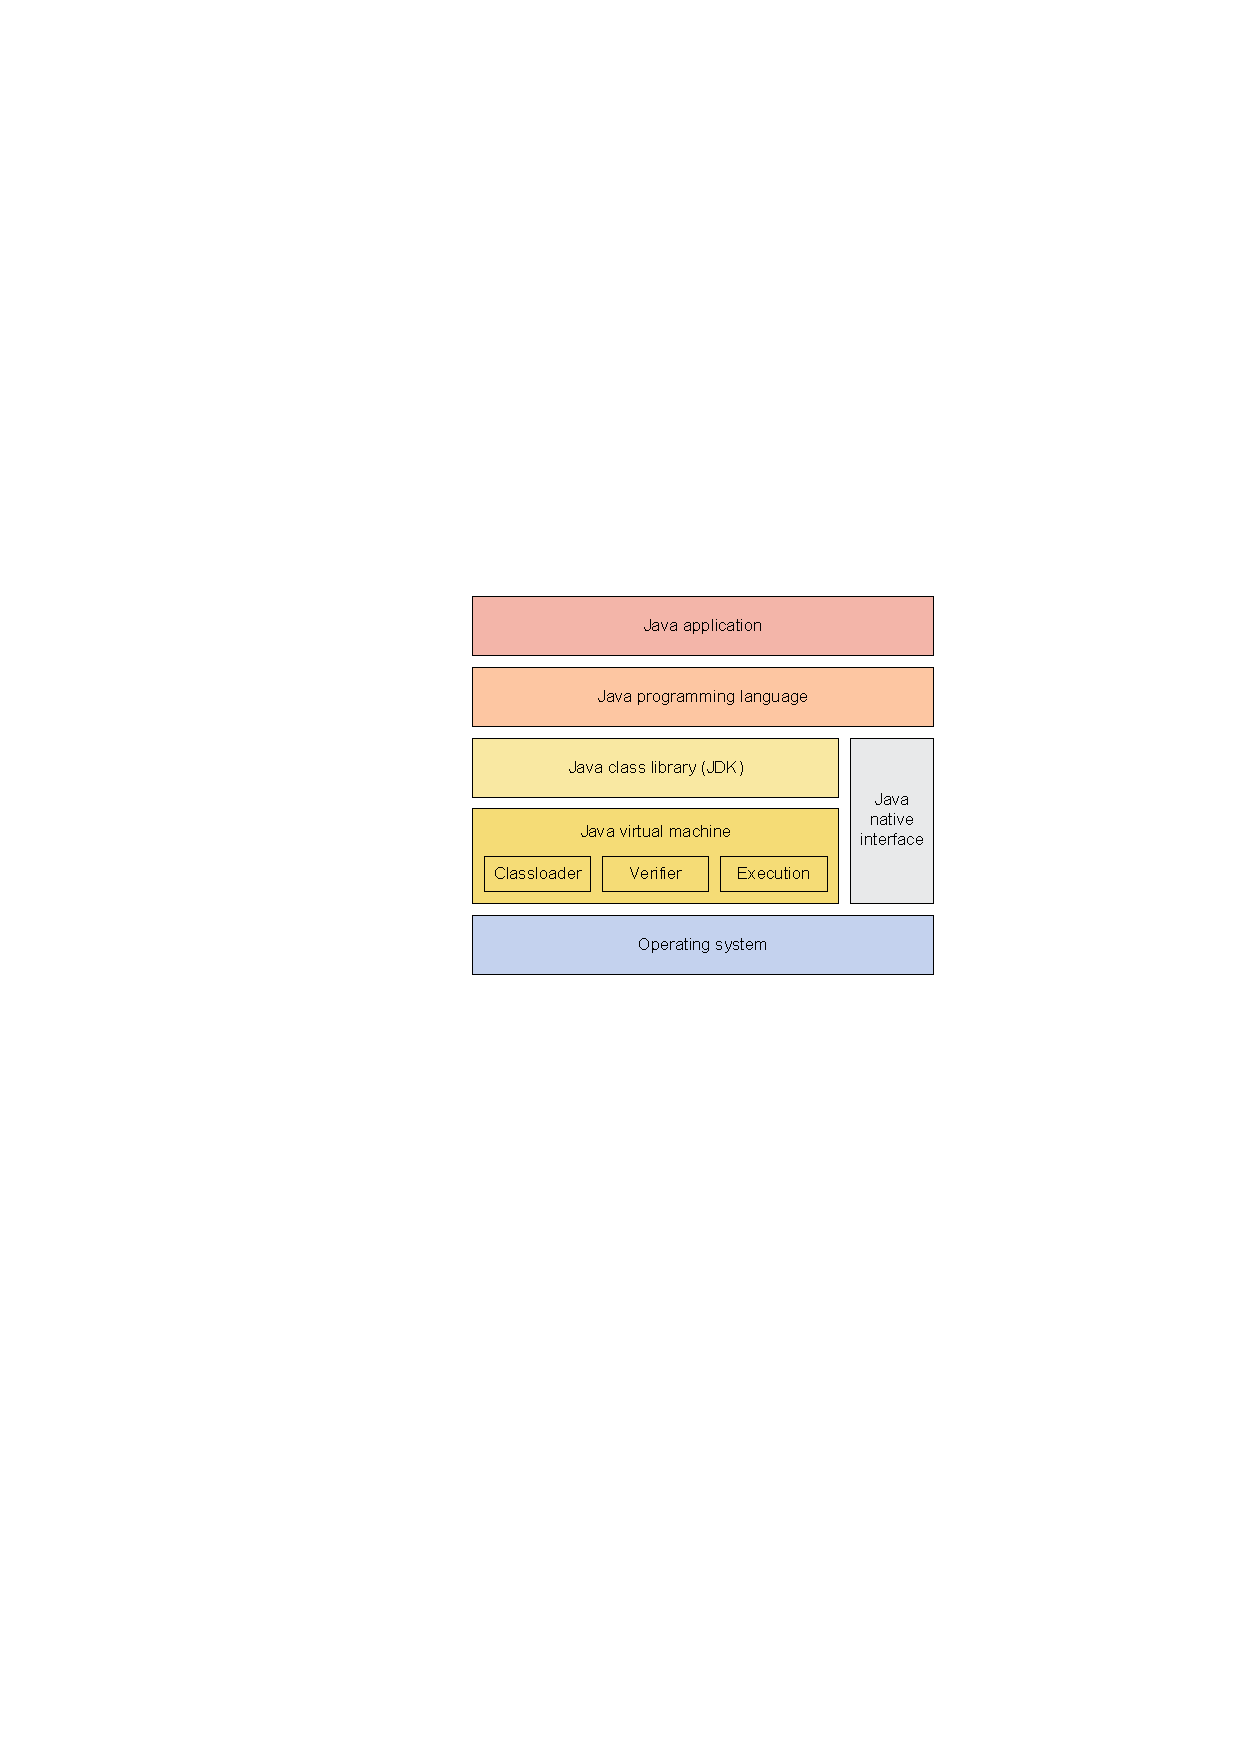
\includegraphics[scale=\picscale]{intro/java_overview}
    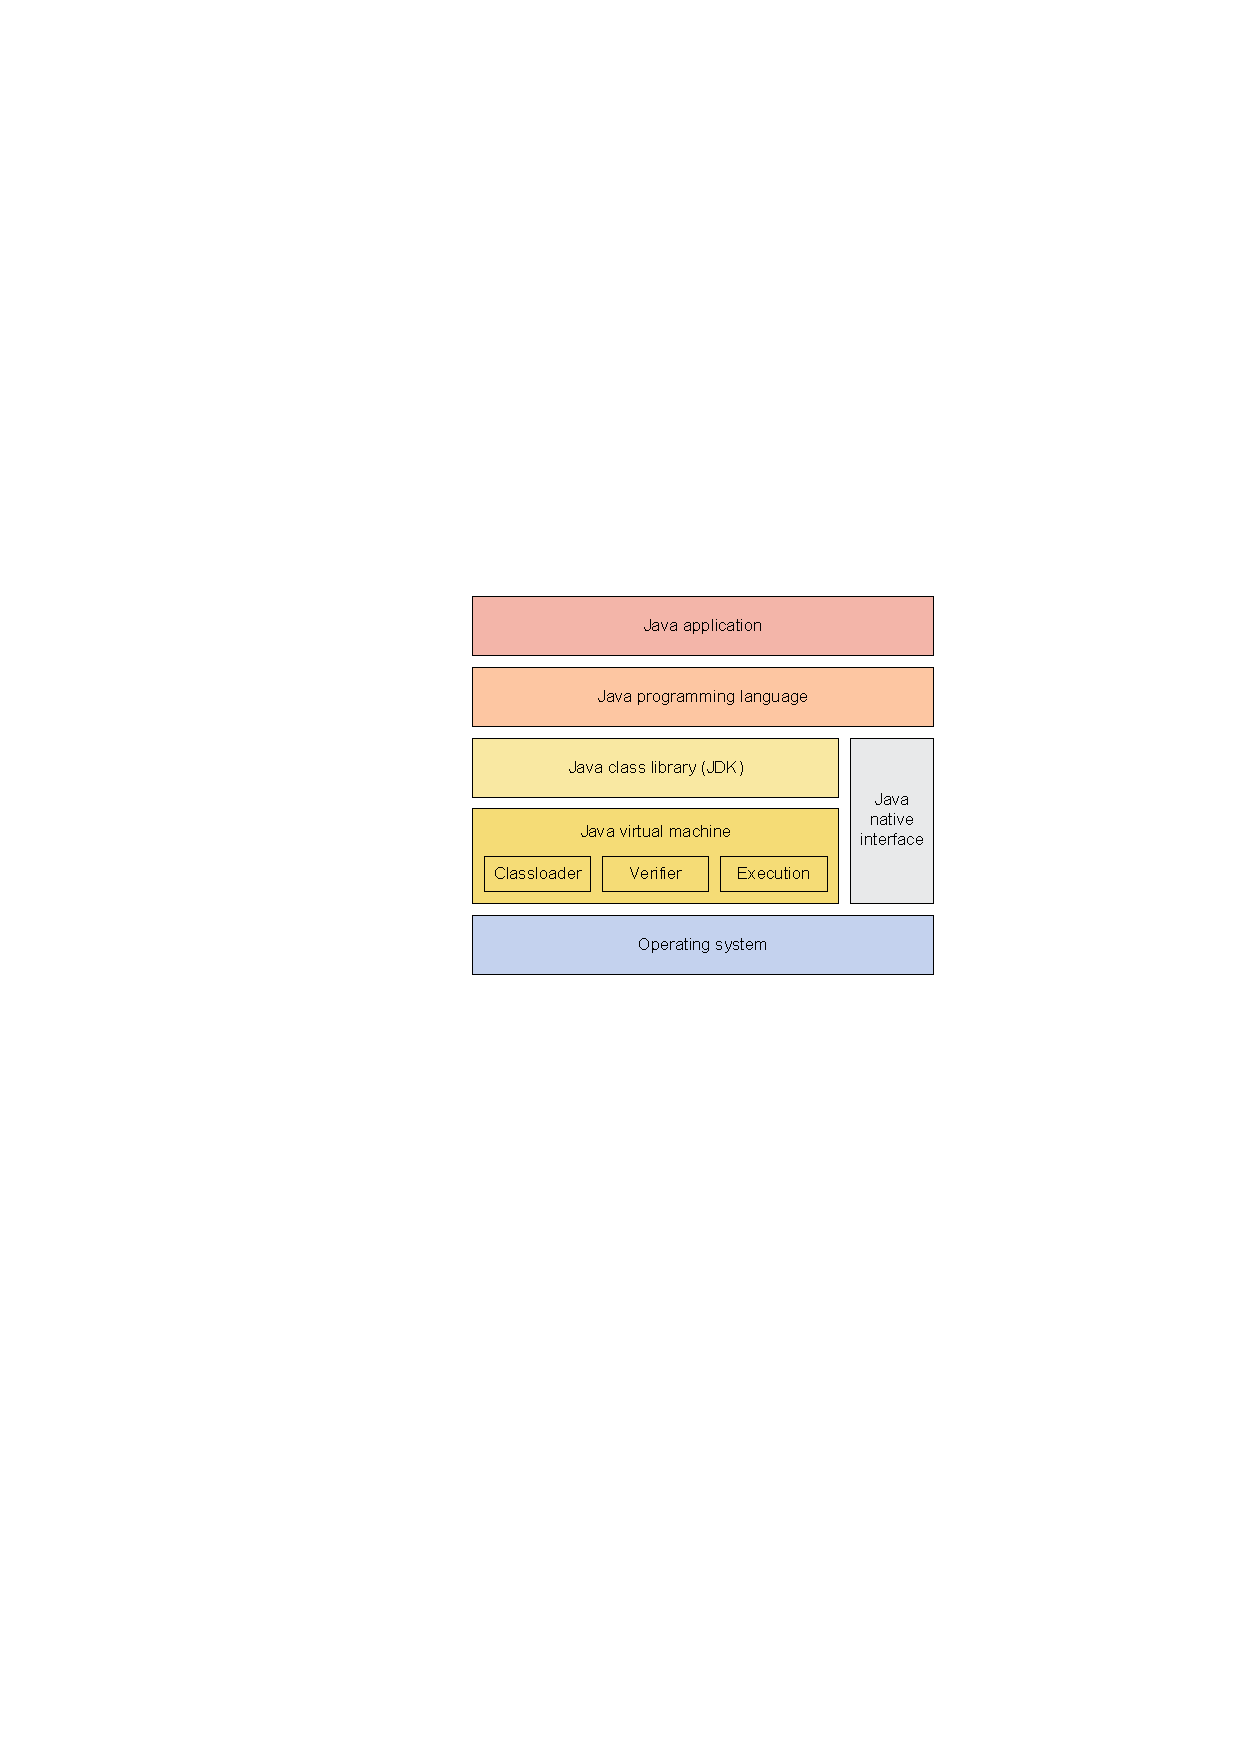
\includegraphics{intro/java_overview}
    \caption{Java system overview}
    \label{fig:java:overview}
\end{figure*}
%
As can be seen in \figurename~\ref{fig:java:overview}, Java consists
of three main components:
%
\begin{enumerate}
    \item The Java programming language as defined in
    \cite{JavaLangSpec2}
    \item The class library, defined as part of the Java
        specification. All implementations of Java have to
        contain the library as defined by Sun
    \item The Java virtual machine (defined in \cite{jvm}) that loads,
     verifies and executes the binary representation (the
\emph{class file}) of a Java program
\end{enumerate}
%
The Java native interface supports functions written in C or C++.
This combination is sometimes called \emph{Java technology} to
emphasize the fact that Java is more than just another
object-oriented language.

However, a number of issues have slowed down the broad acceptance of
Java. The original presentation of Java as an Internet language led
to the misconception that Java was not a general-purpose programming
language. Another obstacle was the first implementation of the JVM as
an interpreter. Execution of Java programs was \emph{very} slow
compared to compiled C/C++ programs. Although advances in its runtime
technology, in particular the just-in-time compiler, have closed the
performance gap, it is still a commonly held view that Java is slow.

\subsection{History}



The Java programming language originated as part of the Green project
specifically for an embedded device, a handheld wireless PDA. In the
early '90s, Java, which was originally known as Oak \cite{java:oak,
java:oak2}, was created as the programming tool for this device. The
device (known as *7) was a small SPARC-based hardware device with a
tiny embedded OS. However, the *7 was never released as a product and
Java was officially released in 1995 as the \emph{new} language for
the Internet. Over the years, Java technology has become a
programming tool for desktop applications, web servers and server
applications. These application domains resulted in the split of the
Java platform into the Java standard edition (J2SE) and the
enterprise edition (J2EE) in 1999. With every new release, the
library (defined as part of the language) continued to grow. Java for
embedded systems was clearly not an area Sun was interested in
pursuing. However, with the arrival of mobile phones, Sun again
became interested in this embedded market. Sun defined different
subsets of Java, which have now been combined into the Java Micro
Edition (J2ME).

In 1999, a document defining the requirements for real-time Java was
published by the NIST \cite{nist99}. Based on these requirements, two
groups defined specifications for real-time Java: the Real-Time Core
Extension \cite{JCons00} published under the J~Consortium and the
Real-Time Specification for Java (RTSJ) \cite{rtsj}. A comparison of
these two specifications and a comparison with Ada 95's Real-Time
Annex can be found in \cite{507579}. The RTSJ was the first Java
Specification Request (JSR 1) under the Java Community Process (JCP)
and started 1999. The first release came out 2002 and further
enhancement of the RTSJ (to version 1.1) are covered by the JSR~282
(started in 2005). Under JSR~302 (Safety Critical Java Technology) a
subset of the RTSJ is currently defined for the safety critical
domain (e.g., standard DO-178B/ED-12B \cite{do-178b}). A detailed
description of the J2ME and specifications for real-time Java can be
found in Chapter~4 of \cite{jop:thesis}.

\subsection{The Java Programming Language}

The Java programming language is a general-purpose object-oriented
language. Java is related to C and C++, but with a number of aspects
omitted. Java is a strongly typed language, which means that type
errors can be detected at compile time. Other errors, such as wrong
indices in an array, are checked at runtime. The
problematic\footnote{C pointers represent memory addresses as data.
Pointer arithmetic and direct access to memory leads to common and
hard-to-find program errors.} \emph{pointer} in C and explicit
deallocation of memory is completely avoided. The pointer is replaced
by a \emph{reference}, i.e., an abstract pointer to an object.
Storage for an object is allocated from the heap during creation of
the object with \code{new}. Memory is freed by automatic storage
management, typically using a garbage collector. The garbage
collector avoids memory leaks from a missing \code{free()} and the
safety problems exposed by dangling pointers.

The types in Java are divided into two categories: primitive types
and reference types. \tablename~\ref{tab:java:primitive} lists the
available primitive types. Method local variables, class fields and
object fields contain either a primitive type value or a reference
to an object.

\begin{table}
    \centering
    \begin{tabular}{ll}
        \toprule
        Type & Description \\
        \midrule
        \code{boolean} & either \code{true} or \code{false} \\
        \code{char} & 16-bit Unicode character (unsigned) \\
        \code{byte} & 8-bit integer (signed) \\
        \code{short} & 16-bit integer (signed) \\
        \code{int} & 32-bit integer (signed) \\
        \code{long} & 64-bit integer (signed) \\
        \code{float} & 32-bit floating-point (IEEE 754-1985) \\
        \code{double} & 64-bit floating-point (IEEE 754-1985) \\
        \bottomrule
    \end{tabular}
    \caption{Java primitive data types}
    \label{tab:java:primitive}
\end{table}

Classes and class instances, the objects, are the fundamental data
and code organization structures in Java. There are no global
variables or functions as there are in C/C++. Each method belongs to
a class. This `everything belongs to a class or an object' combined
with the class naming convention, as suggested by Sun, avoids name
conflicts in even the largest applications.

New classes can extend exactly one superclass. Classes that do not
explicitly extend a superclass become direct subclasses of
\code{Object}, the root of the whole class tree. This single
inheritance model is extended by \emph{interfaces}. Interfaces are
abstract classes that only define method signatures and provide no
implementation. A concrete class can implement several interfaces.
This model provides a simplified form of multiple inheritance.

Java supports multitasking through \emph{threads}. Each thread is a
separate flow of control, executing concurrently with all other
threads. A thread contains the method stack as thread local data --
all objects are shared between threads. Access conflicts to shared
data are avoided by the proper use of \code{synchronized} methods or
code blocks.

Java programs are compiled to a machine-independent bytecode
representation as defined in \cite{jvm}. Although this intermediate
representation is defined for Java, other programming languages
(e.g., ADA \cite{269646}) can also be compiled into Java bytecodes.

\section{The Java Virtual Machine}

The Java virtual machine (JVM) is a definition of an abstract
computing machine that executes bytecode programs. The JVM
specification \cite{jvm} defines three elements:
\begin{itemize}
    \item An instruction set and the meaning of those instructions
    -- the \emph{bytecodes}
    \item A binary format -- the \emph{class file} format. A
    class file contains the bytecodes, a symbol table and other
    ancillary information
    \item An algorithm to \emph{verify} that a class file
    contains valid programs
\end{itemize}
%
In the solution presented in this book, the class files are
verified, linked and transformed into an internal representation
before being executed on JOP. This transformation is performed with
\cmd{JOPizer} and is not executed on JOP. We will therefore omit the
description of the class file and the verification process.

The instruction set of the JVM is stack-based. All operations take
their arguments from the stack and put the result onto the stack.
Values are transferred between the stack and various memory areas.
We will discuss these memory areas first, followed by an explanation
of the instruction set.

\subsection{Memory Areas}

The JVM contains various runtime data areas. Some of these areas are
shared between threads, whereas other data areas exist separately
for each thread.

\begin{description}
    \item[Method area:]
The method area is shared among all threads. It contains static
class information such as field and method data, the code for the
methods and the constant pool. The constant pool is a per-class
table, containing various kinds of constants such as numeric values
or method and field references. The constant pool is similar to a
symbol table.

Part of this area, the code for the methods, is very frequently
accessed (during instruction fetch) and therefore is a good
candidate for caching.

    \item[Heap:]
The heap is the data area where all objects and arrays are
allocated. The heap is shared among all threads. A garbage collector
reclaims storage for objects.

    \item[JVM stack:]
Each thread has a private stack area that is created at the same
time as the thread. The JVM stack is a logical stack that contains
following elements:
\begin{enumerate}
    \item A frame that contains return information for a method
    \item A local variable area to hold local values inside a method
    \item The operand stack, where all operations are performed
\end{enumerate}
%
Although it is not strictly necessary to allocate all three elements
to the same type of memory we will see in Section~\ref{sec:stack}
that the argument-passing mechanism regulates the layout of the JVM
stack.

Local variables and the operand stack are accessed as frequently
as registers in a standard processor. A Java processor should
provide some caching mechanism of this data area.

\end{description}
%
The memory areas are similar to the various segments in conventional
processes (e.g.\ the method code is analogous to the `text'
segment). However, the operand stack replaces the registers in a
conventional processor.

\subsection{JVM Instruction Set}

The instruction set of the JVM contains 201 different instructions
\cite{jvm}. This \emph{bytecodes} can be grouped into the following
categories:
%
\begin{description}
    \item[Load and store:]
Load instructions push values from the local variables onto the
operand stack. Store instructions transfer values from the stack
back to local variables. 70 different instructions belong to this
category. Short versions (single byte) exist to access the first
four local variables. There are unique instructions for each basic
type (\code{int}, \code{long}, \code{float}, \code{double} and
\code{reference}). This differentiation is necessary for the
bytecode verifier, but is not needed during execution. For example
\code{iload}, \code{fload} and \code{aload} all transfer one 32-bit
word from a local variable to the operand stack.

    \item[Arithmetic:]
The arithmetic instructions operate on the values found on the stack
and push the result back onto the operand stack. There are
arithmetic instructions for \code{int}, \code{float} and
\code{double}. There is no direct support for \code{byte},
\code{short} or \code{char} types. These values are handled by
\code{int} operations and have to be converted back before being
stored in a local variable or an object field.

    \item[Type conversion:] The type conversion instructions
        perform numerical conversions between all Java types: as
        implicit widening conversions (e.g., \code{int} to
        \code{long}, \code{float} or \code{double}) or explicit
        (by casting to a type) narrowing conversions.

    \item[Object creation and manipulation:]
Class instances and arrays (that are also objects) are created and
manipulated with different instructions. Objects and class fields
are accessed with type-less instructions.

    \item[Operand stack manipulation:]
All direct stack manipulation instructions are type-less and
operate on 32-bit or 64-bit entities on the stack. Examples of these
instructions are \code{dup}, to duplicate the top operand stack
value, and \code{pop}, to remove the top operand stack value.

    \item[Control transfer:]
Conditional and unconditional branches cause the JVM to continue
execution with an instruction other than the one immediately
following. Branch target addresses are specified relative to the
current address with a signed 16-bit offset. The JVM provides a
complete set of branch conditions for \code{int} values and
references. Floating-point values and type \code{long} are
supported through compare instructions. These compare instructions
result in an \code{int} value on the operand stack.

    \item[Method invocation and return:]
The different types of methods are supported by four instructions:
invoke a class method, invoke an instance method, invoke a method
that implements an interface and an \code{invokespecial} for an
instance method that requires special handling, such as
\code{private} methods or a superclass method.


\end{description}
%
A bytecode consists of one instruction byte followed by optional
operand bytes. The length of the operand is one or two bytes, with
the following exceptions: \code{multianewarray} contains 3 operand
bytes; \code{invokeinterface} contains 4 operand bytes, where one is
redundant and one is always zero; \code{lookupswitch} and
\code{tableswitch} (used to implement the Java \code{switch}
statement) are variable-length instructions; and \code{goto\_w} and
\code{jsr\_w} are followed by a 4 byte branch offset, but neither is
used in practice as other factors limit the method size to 65535
bytes.

\subsection{Methods}

A Java \emph{method} is equivalent to a \emph{function} or
\emph{procedure} in other languages. In object oriented terminology
this \emph{method} is \emph{invoked} instead of \emph{called}. We
will use \emph{method} and \emph{invoke} in the remainder of this
text. In Java and the JVM, there are five types of methods:
%
\begin{itemize}
    \item Static or class methods
    \item Virtual methods
    \item Interface methods
    \item Class initialization
    \item Constructor of the parent class (\code{super()})
\end{itemize}
%
For these five types there are only four different bytecodes:
\begin{description}
    \item[\code{invokestatic}:] A class method (declared \code{static})
    is invoked. As the target does not depend on an object, the
    method reference can be resolved at load/link time.

    \item[\code{invokevirtual}:] An object reference is resolved and
    the corresponding method is invoked. The resolution is usually
    done with a dispatch table per class containing all implemented and
    inherited methods. With this dispatch table, the resolution can
    be performed in constant time.

    \item[\code{invokeinterface}:] An interface allows Java
    to emulate multiple inheritance. A class can implement several
    interfaces, and different classes (that have no inheritance
    relation) can implement the same interface. This flexibility
    results in a more complex resolution process. One method of
    resolution is a search through the class hierarchy that results
    in a variable, and possibly lengthy, execution time. A constant time
    resolution is possible by assigning every interface method a
    unique number. Each class that implements an interface needs its
    own table with unique positions for each interface method of
    the \emph{whole} application.

    \item[\code{invokespecial}:] Invokes an instance method with
    special handling for superclass, \code{private}, and instance
    initialization. This bytecode catches many different cases.
    This results in expensive checks for common \code{private} instance
    methods.
\end{description}
%

\subsection{Implementation of the JVM}

There are several different ways to implement a virtual machine. The
following list presents these possibilities and analyses how
appropriate they are for embedded devices.
%
\begin{description}
    \item[Interpreter:]
The simplest realization of the JVM is a program that interprets the
bytecode instructions. The interpreter itself is usually written in
C and is therefore easy to port to a new computer system. The
interpreter is very compact, making this solution a primary choice
for resource-constrained systems. The main disadvantage is the high
execution overhead. From a code fragment of the typical interpreter
loop, as shown in Listing~\ref{lst:intro:java:intprt}, we can
examine the overhead: The emulation of the stack in a high-level
language results in three memory accesses for a simple \code{iadd}
bytecode. The instruction is decoded through an indirect jump.
Indirect jumps are still a burden for standard branch prediction
logic.

\begin{lstlisting}[float,caption={A typical JVM interpreter loop},
label=lst:intro:java:intprt]
    for (;;) {
        instr = bcode[pc++];
        switch (instr) {
            ...
            case IADD:
                tos = stack[sp]+stack[sp-1];
                --sp;
                stack[sp] = tos;
                break;
            ...
        }
    }
\end{lstlisting}

    \item[Just-In-Time Compilation:]
Interpreting JVMs can be enhanced with just-in-time (JIT) compilers.
A JIT compiler translates Java bytecodes to native instructions
during runtime. The time spent on compilation is part of the
application execution time. JIT compilers are therefore restricted
in their optimization capacity. To reduce the compilation overhead,
current JVMs operate in mixed mode: Java methods are executed in
interpreter mode and the call frequency is monitored. Often-called
methods, the hot spots, are then compiled to native code.

JIT compilation has several disadvantages for embedded systems,
notably that a compiler (with the intrinsic memory overhead) is
necessary on the target system. Due to compilation during
runtime, execution times are hardly predictable.\footnote{Even if
the time for the compilation is known, the WCET for a method has
to include the compile time! Furthermore, WCET analysis has to
know in advance what code will be produced by JIT compilation.}

    \item[Batch Compilation:]
Java can be compiled, in advance, to the native instruction set of
the target. Precompiled libraries are linked with the application
during runtime. This is quite similar to C/C++ applications with
shared libraries. This solution undermines the flexibility of Java:
dynamic class loading during runtime. However, this is not a major
concern for embedded systems.


    \item[Hardware Implementation:] A Java processor is the
        implementation of the JVM in hardware. The JVM bytecode
        is the native instruction set of such a processor. This
        solution can result in quite a small processor, as a
        stack architecture can be implemented very efficiently. A
        Java processor is memory-efficient as an interpreting
        JVM, but avoids the execution overhead. The main
        disadvantage of a Java processor is the lack of
        capability to execute C/C++ programs. This book describes
        JOP as an example of a JVM hardware implementation.

\end{description}

\section{Embedded Java}

\begin{figure}
    \centering
    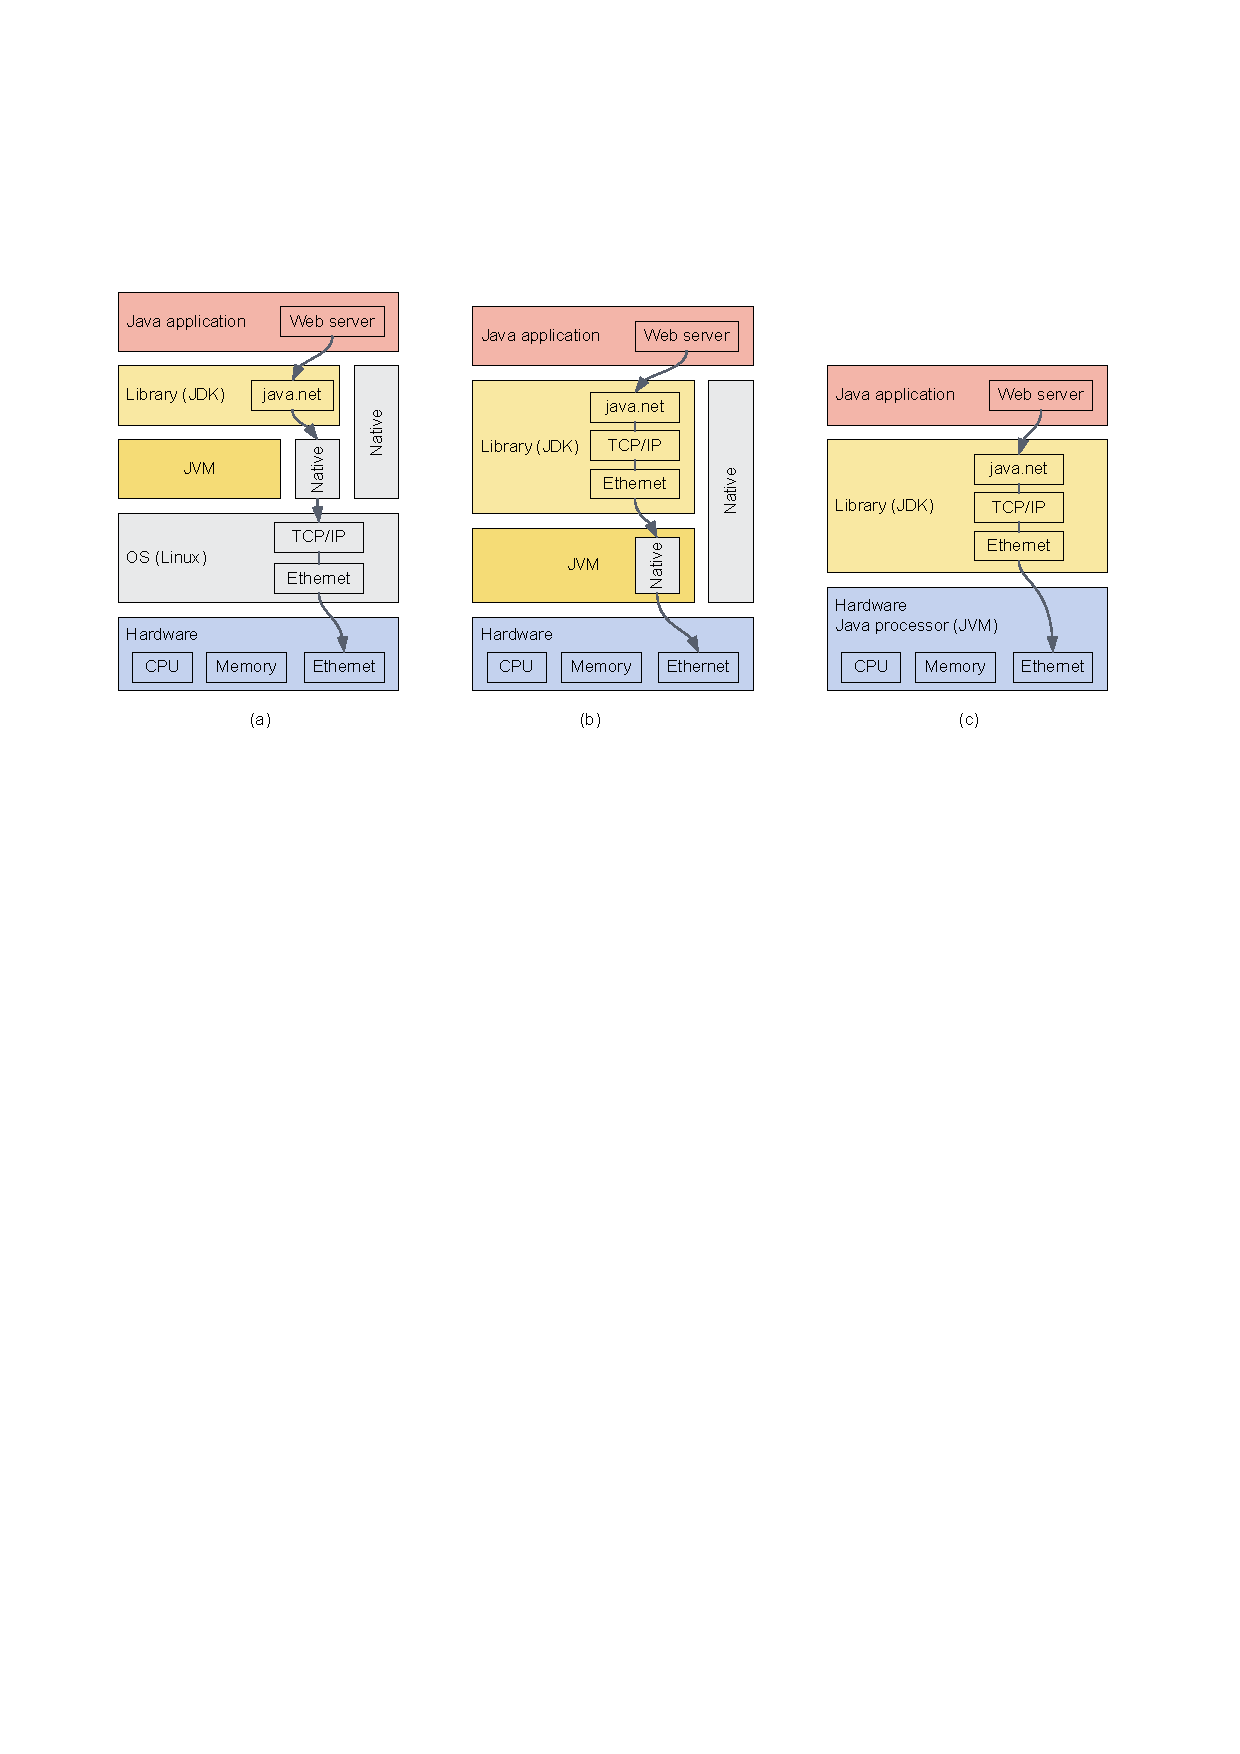
\includegraphics[width=\textwidth]{intro/jvmall}
    \caption{Implementation variations for an embedded JVM: (a) standard layers
    for Java with an operating system -- equivalent to desktop configurations, (b) a JVM on the bare metal,
    and (c) a JVM as a Java processor.}\label{fig:java:embedded}
\end{figure}

In embedded systems the architecture of JVMs are more diverse than
on desktop or server systems. Figure~\ref{fig:java:embedded} shows
variations of Java implementations in embedded systems and an
example of the control flow for a web server application. The
standard approach of a JVM running on top of an operating system
(OS) is shown in sub-figure (a). A network connection bypasses the
JVM via native functions and uses the TCP/IP stack implementation
and the device drivers of the OS.

A JVM without an OS is shown in sub-figure (b). This solution is
often called \emph{running on the bare metal}. The JVM acts as the OS
and provides the thread scheduling and the low-level access to the
hardware. In that case the network stack can be written entirely in
Java. JNode\footnote{\url{http://www.jnode.org/}} is an approach to
implement the OS entirely in Java. This solution becomes popular even
in server applications.\footnote{BEA System offers the JVM LiquidVM
that includes basic OS functions and does not need a guest OS.
%\url{http://www.bea.com/framework.jsp?CNT=index.htm&FP=/content/products/weblogic/virtual_server}
}

Sub-figure (c) shows an embedded solution where the JVM is part of
the hardware layer. That means it is implemented in a Java
processor. With this solution the native layer can be completely
avoided and all code (application and system code) is written
entirely in Java.

Figure~\ref{fig:java:embedded} shows how the flow from the
application goes down to the hardware. The example consists of a web
server and an Internet connection via Ethernet. In case (a) the
application web server talks with \code{java.net} in the JDK. The
flow goes through a native interface to the TCP/IP implementation and
the Ethernet device driver within the OS (usually written in C). The
device driver talks with the Ethernet chip. In (b) the OS layer is
omitted: the TCP/IP layer and the Ethernet device driver are now part
of the Java library. In (c) the JVM is part of the hardware layer and
a direct access from the Ethernet driver to the Ethernet hardware is
mandatory. Note how part of the network stack moves up from the OS
layer to the Java library. Version (c) shows a pure Java
implementation of the whole network stack.


%% This section can be found in the thesis. If we want to have such
%% a section in the handbook we should change it and add more interesting
%% numbers. Also redo the Excel graphs.

%\section{Benchmarking the JVM}
%\label{sec:bench:jvm}
%
%The rationale behind this section is best introduced with a warning
%from Computer Architecture: A Quantitative Approach \cite{Hennessy02}
%p. 63:
%
%\begin{quote}
%Virtually every practicing computer architect knows Amdahl�s Law.
%Despite this, we almost all occasionally fall into the trap of
%expending tremendous effort optimizing some aspect of a system before
%we measure its usage. Only when the overall speedup is unrewarding do
%we recall that we should have measured the usage of that feature
%before we spent so much effort enhancing it!
%\end{quote}
%%
%We measured how Java programs use the bytecode instruction set and
%explored the typical and worst-case method sizes. Our measurements
%and other reports are presented in the following sections.
%
%\subsection{Bytecode Frequency}
%
%The dynamic instruction frequency is the main measurement for
%determining a processor implementation. We can identify those
%instructions that should be fast. For seldom-used instructions, a
%trade-off can be made between performance and hardware resources.
%
%Many reports have been written about JVM bytecode frequencies (e.g.\
%\cite{Greg2002, 365338, pJ1}). Most of these reports provide only a
%coarse categorization of the bytecodes. For example, the bytecodes
%\code{iload\_n} (load an \code{int} from a local variable) and
%\code{getfield} (fetch a field from an object) are combined in one
%instruction category. However, these instructions are very different
%in terms of their implementation complexity. We have chosen a
%fine-grained categorization of the bytecodes to gain greater insight
%into the bytecode usage. In Table~\ref{tab_java_instr_cat} all 201
%bytecode instructions are listed by category.
%
%
%\begin{table}
%    \centering
%    \begin{tabular}{ll}
%    \toprule
%    Type & Bytecode \\
%    \midrule
%
%    load
%    & aload, dload, fload, iload, lload \\
%
%    load (short)
%    & aload\_0, aload\_1, aload\_2, aload\_3, \\
%    & dload\_0, dload\_1, dload\_2, dload\_3, \\
%    & fload\_0, fload\_1, fload\_2, fload\_3, \\
%    & iload\_0, iload\_1, iload\_2, iload\_3, \\
%    & lload\_0, lload\_1, lload\_2, lload\_3 \\
%
%    store
%    & astore, dstore, fstore, istore, lstore \\
%
%    store (short)
%    & astore\_0, astore\_1, astore\_2, astore\_3, \\
%    & dstore\_0, dstore\_1, dstore\_2, dstore\_3, \\
%    & fstore\_0, fstore\_1, fstore\_2, fstore\_3, \\
%    & istore\_0, istore\_1, istore\_2, istore\_3, \\
%    & lstore\_0, lstore\_1, lstore\_2, lstore\_3 \\
%
%    const
%    & bipush, ldc, ldc\_w, ldc2\_w, sipush \\
%
%    const (short)
%    & aconst\_null, dconst\_0, dconst\_1, fconst\_0, fconst\_1, fconst\_2, \\
%    & iconst\_0, iconst\_1, iconst\_2, iconst\_3, iconst\_4, iconst\_5, \\
%    & iconst\_m1, lconst\_0, lconst\_1 \\
%
%    get
%    & getfield, getstatic \\
%
%    put
%    & putfield, putstatic \\
%
%    alu
%    & dadd, ddiv, dmul, dneg, drem, dsub, \\
%    & fadd, fdiv, fmul, fneg, frem, fsub, \\
%    & iadd, iand, idiv, imul, ineg, ior, irem, ishl, ishr, isub, iushr, ixor, \\
%    & ladd, land, ldiv, lmul, lneg, lor, lrem, lshl, lshr, lsub, lushr, lxor \\
%
%    iinc
%    & iinc \\
%
%    stack
%    & dup, dup\_x1, dup\_x2, dup2, dup2\_x1, dup2\_x2, pop, pop2, swap \\
%
%    array
%    & aaload, aastore, baload, bastore, caload, castore, daload, dastore, \\
%    & faload, fastore, iaload, iastore, laload, lastore, saload, sastore \\
%
%    branch
%    & goto, goto\_w, if\_acmpeq, if\_acmpne, if\_icmpeq, \\
%    & if\_icmpge, if\_icmpgt, if\_icmple, if\_icmplt, if\_icmpne, \\
%    & ifeq, ifge, ifgt, ifle, iflt, ifne, ifnonnull, ifnull \\
%
%    compare
%    & dcmpg, dcmpl, fcmpg, fcmpl, lcmp \\
%
%    switch
%    & lookupswitch, tableswitch \\
%
%    call
%    & invokeinterface, invokespecial, invokestatic, invokevirtual \\
%
%    return
%    & areturn, dreturn, freturn, ireturn, lreturn, return \\
%
%    conversion
%    & d2f, d2i, d2l, f2d, f2i, f2l, i2b, i2c, i2d, i2f, i2l, i2s, l2d, l2f, l2i \\
%
%    new
%    & anewarray, multianewarray, new, newarray \\
%
%    other
%    & arraylength, athrow, checkcast, instanceof, jsr, jsr\_w, \\
%    & monitorenter, monitorexit, nop, ret, wide \\
%
%
%    \bottomrule
%    \end{tabular}
%    \caption[Categories of JVM bytecodes]{The 201 Java bytecodes and
%    their assignment to different categories}
%    \label{tab_java_instr_cat}
%\end{table}
%
%
%Three different applications were run on an instrumented JVM to
%measure dynamic bytecode frequency. The results were compared with
%the results from the above-mentioned reports. In
%Table~\ref{tab_java_instr_frequ} the dynamic instruction count for
%the three different benchmarks is shown. The last column is the
%average of the three tests weighted by the individual instructions
%count.
%
%Kaffe \cite{kaffe} is an independent implementation of the JVM
%distributed under the GNU Public License. Kaffe was instrumented to
%collect the data on dynamic bytecode usage. Three different
%applications were used as benchmarks to obtain the dynamic
%instruction count: JLex, KCJ and javac. JLex \cite{jlex} is a lexical
%analyzer generator, written for Java in Java. The data was collected
%by running JLex with the provided \code{sample.lex} as the input
%file. KJC \cite{kcj} is a Java compiler in Java, freely available
%under the terms of the GNU General Public License. javac is the Sun
%Java compiler. Both compilers were compiling part of the KJC sources
%during the benchmark. These benchmarks are similar to the benchmarks
%used in other reports and the results are therefore comparable.
%However, typical embedded applications can result in a slightly
%different instruction set usage pattern. Embedded applications are
%usually tightly connected with the environment and are therefore not
%available as stand-alone programs to serve as benchmarks. An embedded
%application developed on JOP was adapted to serve as a benchmark for
%Section~\ref{sec:cache} and Chapter~\ref{chap:results}.
%
%%19,572,165 + 951,138,375 + 341,926,231 = 1,312,636,771
%
%% JLex.Main   kaffe JLex.Main JLex/sample.lex
%% at.dms.kjc.Main:
%%    kaffe -cp kjc-2.1B-bin.jar at.dms.kjc.Main -d classes kopi-2.1B/src/kjc/*.java
%% com.sun.tools.javac.Main:
%%    kaffe -cp /usr/lib/java/lib/tools.jar com.sun.tools.javac.Main -d classes kopi-2.1B/src/kjc/*.java
%%  stops with compile error
%
%
%\begin{table}
%    \centering
%    \begin{tabular}{lrrrr}
%        \toprule
%        & JLex & KJC & javac & Average \\
%        \midrule
%        load (short) & 32.72 & 31.45 & 27.24 & 30.37 \\
%        get & 12.02 & 14.39 & 17.04 & 15.04 \\
%        branch & 11.26 & 10.40 & 10.71 & 10.49 \\
%        invoke & 6.87 & 6.31 & 4.24 & 5.77 \\
%        return & 6.82 & 6.20 & 4.17 & 5.68 \\
%        load & 7.59 & 4.19 & 7.48 & 5.09 \\
%        alu & 2.60 & 4.43 & 4.74 & 4.48 \\
%        const (short) & 4.61 & 4.26 & 4.74 & 4.39 \\
%        array & 4.22 & 4.07 & 3.22 & 3.85 \\
%        put & 0.78 & 2.14 & 3.65 & 2.52 \\
%        iinc & 1.81 & 2.38 & 1.41 & 2.12 \\
%        stack & 1.30 & 2.11 & 2.11 & 2.10 \\
%        store (short) & 2.61 & 2.18 & 1.71 & 2.06 \\
%        other & 1.63 & 2.22 & 1.21 & 1.95 \\
%        const & 0.85 & 1.56 & 2.80 & 1.87 \\
%        store & 2.05 & 0.85 & 1.94 & 1.15 \\
%        conversion & 0.02 & 0.36 & 0.58 & 0.42 \\
%        switch & 0.00 & 0.20 & 0.60 & 0.30 \\
%        new & 0.08 & 0.28 & 0.20 & 0.25 \\
%        compare & 0.14 & 0.03 & 0.22 & 0.08 \\
%        \bottomrule
%    \end{tabular}
%    \caption{Dynamic bytecode frequency in \%}
%    \label{tab_java_instr_frequ}
%\end{table}
%
%\begin{table}
%    \centering
%    \begin{tabular}{lrlr}
%        \toprule
%        \multicolumn{2}{c}{JLex, KJC and javac} &
%        \multicolumn{2}{c}{SPEC and Java Grande} \\
%        \cmidrule(lr){1-2} \cmidrule(lr){3-4}
%        Instruction & Frequency & Instruction & Frequency \\
%        \midrule
%        load (short)  & 30.37 & acnst &  0.07 \\
%        load          &  5.09 & aload & 16.23 \\
%        const (short) &  4.39 & fcnst &  0.33 \\
%        const         &  1.87 & fload &  6.33 \\
%                      &       & icnst &  3.21 \\
%                      &       & iload & 18.06 \\
%        \midrule
%        load \& const & \textbf{41.72}& & \textbf{44.77} \\
%        \midrule
%        get           & 15.04 & field & 11.12 \\
%        put           &  2.52 &       &       \\
%        \midrule
%        field access & \textbf{17.56} & & \textbf{11.12} \\
%        \midrule
%        branch        & 10.49 & cjump &  5.67 \\
%        compare       &  0.08 & ujump &  0.51 \\
%        \midrule
%        control & \textbf{10.57}& & \textbf{6.18} \\
%        \midrule
%        invoke & \textbf{5.77} & fcall &  \textbf{3.63} \\
%        \midrule
%        return &  \textbf{5.68} & retrn &  \textbf{2.07} \\
%        \bottomrule
%    \end{tabular}
%    \caption[Dynamic bytecode frequency comared]
%    {Dynamic bytecode frequency compared with the
%    measurements from \cite{Dowling2002}}
%    \label{tab:java:instr:frequ:comp}
%\end{table}
%
%In \cite{Dowling2002} the relationship between static and dynamic
%instruction frequency of 19 programs from the SPECjvm98
%\cite{SPECJvm98} and Java Grande benchmark suites were measured. The
%bytecodes categories were chosen differently from the above
%measurements, but detailed enough to verify our own measurements.
%\tablename~\ref{tab:java:instr:frequ:comp} shows the average dynamic
%execution frequency in percent\footnote{The values do not add up to
%100\% as only the most significant bytecode categories are shown} of
%selected bytecode categories from the SPEC and Java Grande
%benchmarks, compared with the results obtained by our measurements.
%The numbers in bold are categories or sums of categories that are
%comparable. The frequency of the ``load \& const" instructions is
%very similar to that in our measurements. However, field access,
%control instructions and method invocations are more frequent in our
%measurements. The higher count on field access instructions and
%method invocation can result from a more object oriented programming
%style in our selected applications than in the SPEC and Java Grande
%benchmarks. The big difference, not seen in our measurements, between
%the invoke and return frequency in the SPEC and Java Grande
%benchmarks is not explained in \cite{Dowling2002}.
%
%In all measurements, the load of local variables and constants onto
%the stack accounts for more than 40\% of instructions executed. This
%feature shows that an efficient realization of the local variable
%memory area, the stack and the transfer between these memory areas is
%mandatory.
%
%The next most executed bytecodes (\code{getfield} and
%\code{getstatic}) are the instructions that load an object or class
%field onto the operand stack. To account for these frequent
%instructions, the class layout for the runtime system has to be
%optimized for quick resolution of field addresses (i.e.\ minimum
%memory indirections).
%
%The frequency of branches is comparable with the SPECint2000
%measurements on RISC processors \cite{Hennessy02}. With such a high
%branch frequency, a processor without branch prediction logic is put
%under pressure in terms of pipeline length.
%
%It is interesting to note that there are more method invoke
%instructions than return instructions. Two facts are responsible for
%this difference: native methods are invoked by a bytecode, but the
%return is inside the native methods; and an exception can result in a
%method exit without return.
%
%
%\subsection{Methods Types and Length}
%\label{sec:bench:jvm:methods}
%
%\tablename~\ref{tab_java_meth_type} shows the number of dynamic
%method calls of the Java Grande and \linebreak[4]SPECjvm98
%benchmarks. It can be seen that the distribution of method types
%depends on the application type. Usage of virtual methods and
%interfaces is common in OO programming. Static methods result from
%the simple translation of procedural programs to Java.
%
%\begin{table}
%    \centering
%    \begin{tabular}{lrrrr}
%        \toprule
%         & virtual & special & static & interface \\
%        \midrule
%        Java Grande & 57.1 & 8.7 & 34.2 & 0.0 \\
%        SPEC JVM98 & 81.0 & 10.9 & 2.9 & 5.2 \\
%        \bottomrule
%    \end{tabular}
%    \caption{Types of different dynamic method calls for two benchmarks (from \cite{Power2002})}
%    \label{tab_java_meth_type}
%\end{table}
%
%As a basis for the proposed cache solution in
%Section~\ref{sec:cache}, we will explore the static distribution of
%method sizes. In the JVM, only relative branches are defined. The
%conditional branches and goto have an offset of 16 bits, resulting in
%a practical limit of the method length of 32KB. Although there is a
%goto instruction with a wide index (\emph{goto\_w}) that takes a
%4-byte branch offset, other factors (e.g.\ indices in the exception
%table) limit the size of a method to 65535 bytes.
%
%
%\begin{table}
%    \centering
%    \begin{tabular}{rrrr}
%        \toprule
%        Length & Methods & Percentage & Cumulative \\
%        & & & percentage \\
%        \midrule
%        1 & 1,388 & 1.94 & 1.94 \\
%        2 & 1,580 & 2.21 & 4.16 \\
%        4 & 1,871 & 2.62 & 6.78 \\
%        8 & 16,192 & 22.67 & 29.45 \\
%        16 & 12,363 & 17.31 & 46.76 \\
%        32 & 12,638 & 17.70 & 64.45 \\
%        64 & 11,178 & 15.65 & 80.10 \\
%        128 & 7,287 & 10.20 & 90.31 \\
%        256 & 4,304 & 6.03 & 96.33\\
%        512 & 1,727 & 2.42 & 98.75 \\
%        1,024 & 592 & 0.83 & 99.58 \\
%        2,048 & 175 & 0.25 & 99.83 \\
%        4,096 & 75 & 0.11 & 99.93 \\
%        8,192 & 37 & 0.05 & 99.98 \\
%        16,384 & 11 & 0.02 & 100.00 \\
%        32,768 & 1 & 0.00 & 100.00 \\
%        65,536 & 0 & 0.00 & 100.00 \\
%        \bottomrule
%    \end{tabular}
%    \caption{Static method count of different sizes from the runtime library (JDK 1.4).}
%    \label{tab_java_jdk_static_size}
%\end{table}
%
%In Table~\ref{tab_java_jdk_static_size}, the number of methods of
%different sizes in the Java runtime library (JDK 1.4) is shown. The
%library consists of 71419 methods, the largest being 16706 bytes. The
%size is classified by powers of 2 because we are interested in the
%size of cache memory for complete methods. In the table, the row of,
%for example, size 32 includes all methods of a size from 17 to 32
%bytes. It can be seen that methods are typically very short. In fact,
%99\% of the methods are less than 513 bytes in size. This property is
%important for the proposed method cache in Section~\ref{sec:cache},
%where a complete method has to fit into the instruction cache.
%
%All larger methods are different kinds of initialization functions,
%in most cases \code{$<$clinit$>$()}\footnote{The class or interface
%initialization method is static and the special name
%\codefoot{$<$clinit$>$} is supplied by the compiler. These
%initialization methods are invoked implicitly by the JVM.}. The large
%class initialization methods typically result from the initialization
%of arrays with constant data. This is necessary because of the lack
%of initialized data segments, such as the BSS in C, in the Java class
%file. These initialization methods contain straight-line code and can
%therefore be split to smaller methods automatically, if necessary.
%
%\begin{figure}
%    \centering
%    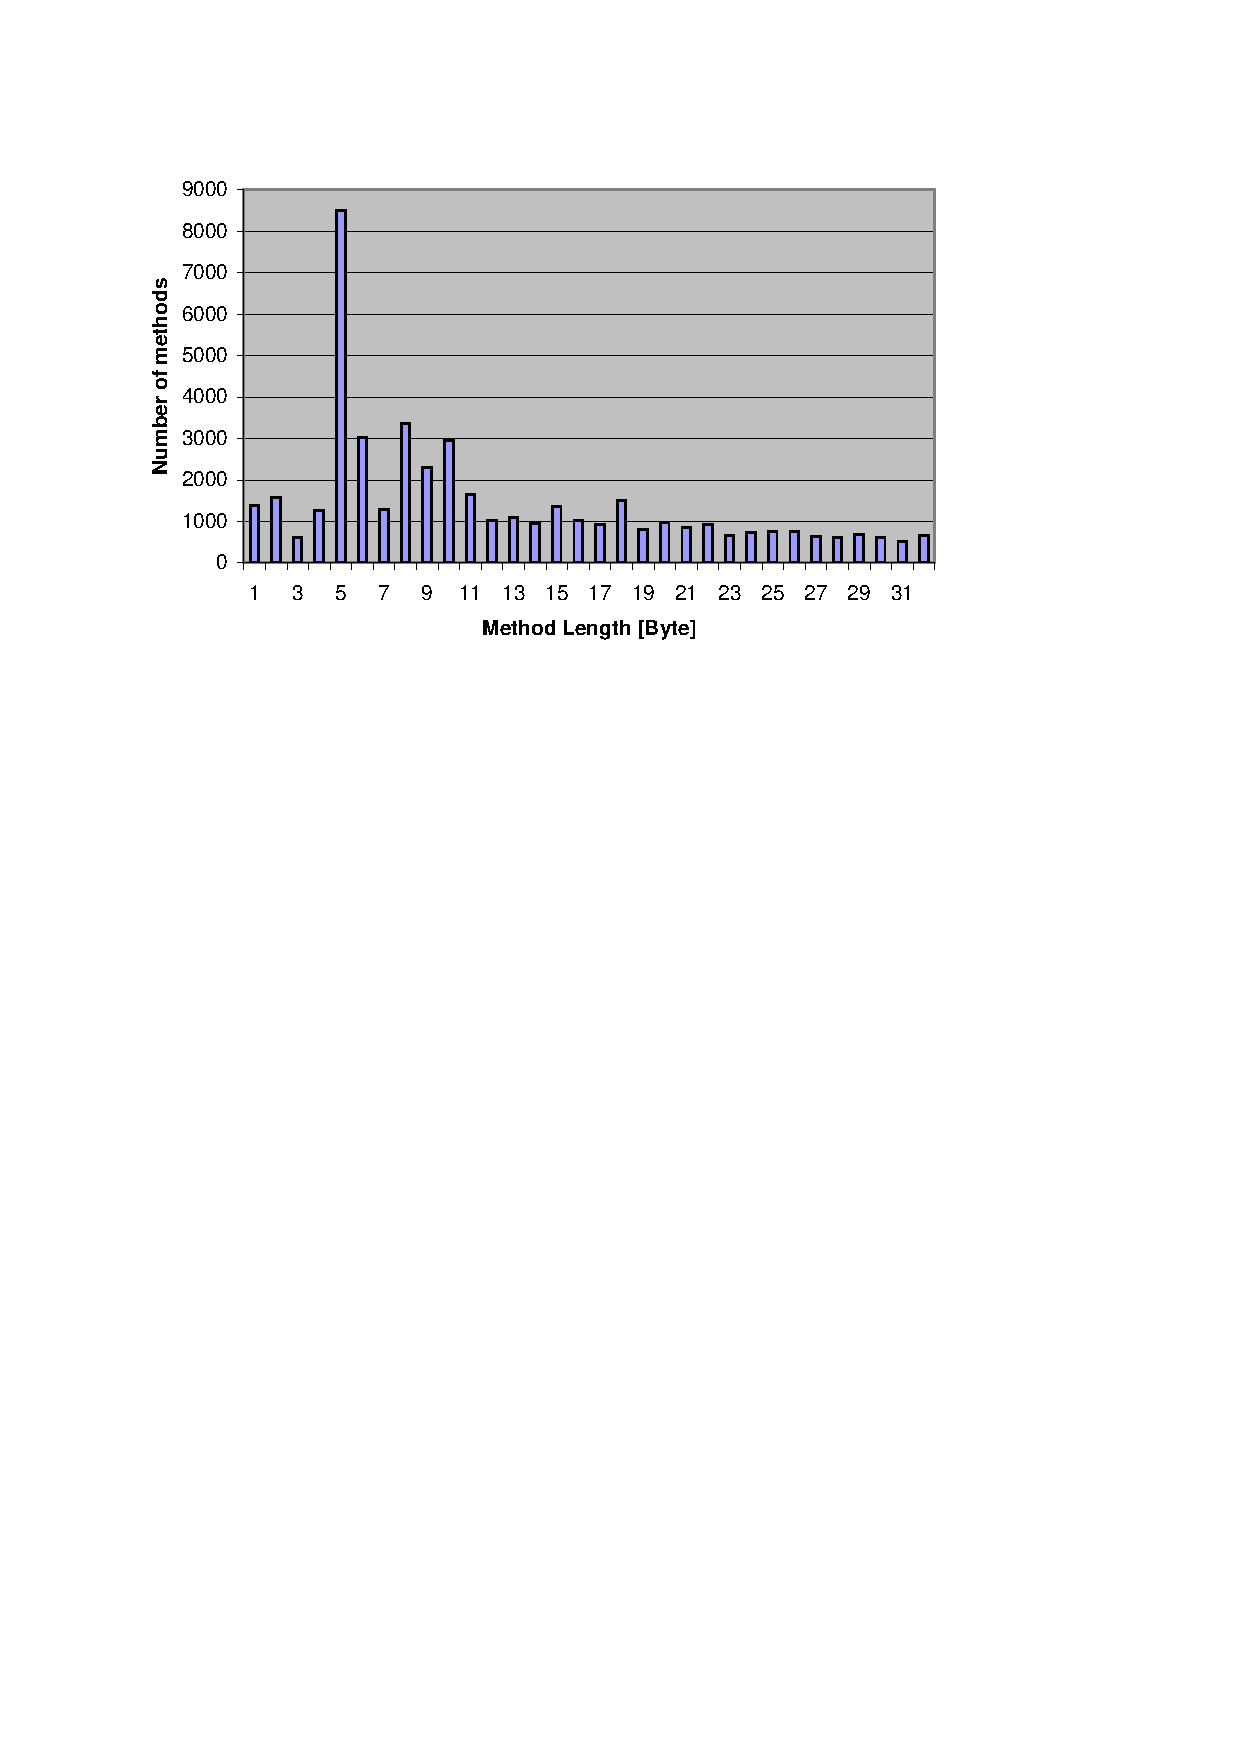
\includegraphics[width=\excelwidth]{arch/arch_meth32}
%    \caption[Static method count for methods of size up to 32 bytes]
%    {Static method count for methods of size up to 32 bytes in the JDK 1.4 runtime library.
%    The horizontal axis indicates the method size.}
%    \label{fig_java_meth32}
%\end{figure}
%
%\begin{figure}
%    \centering
%    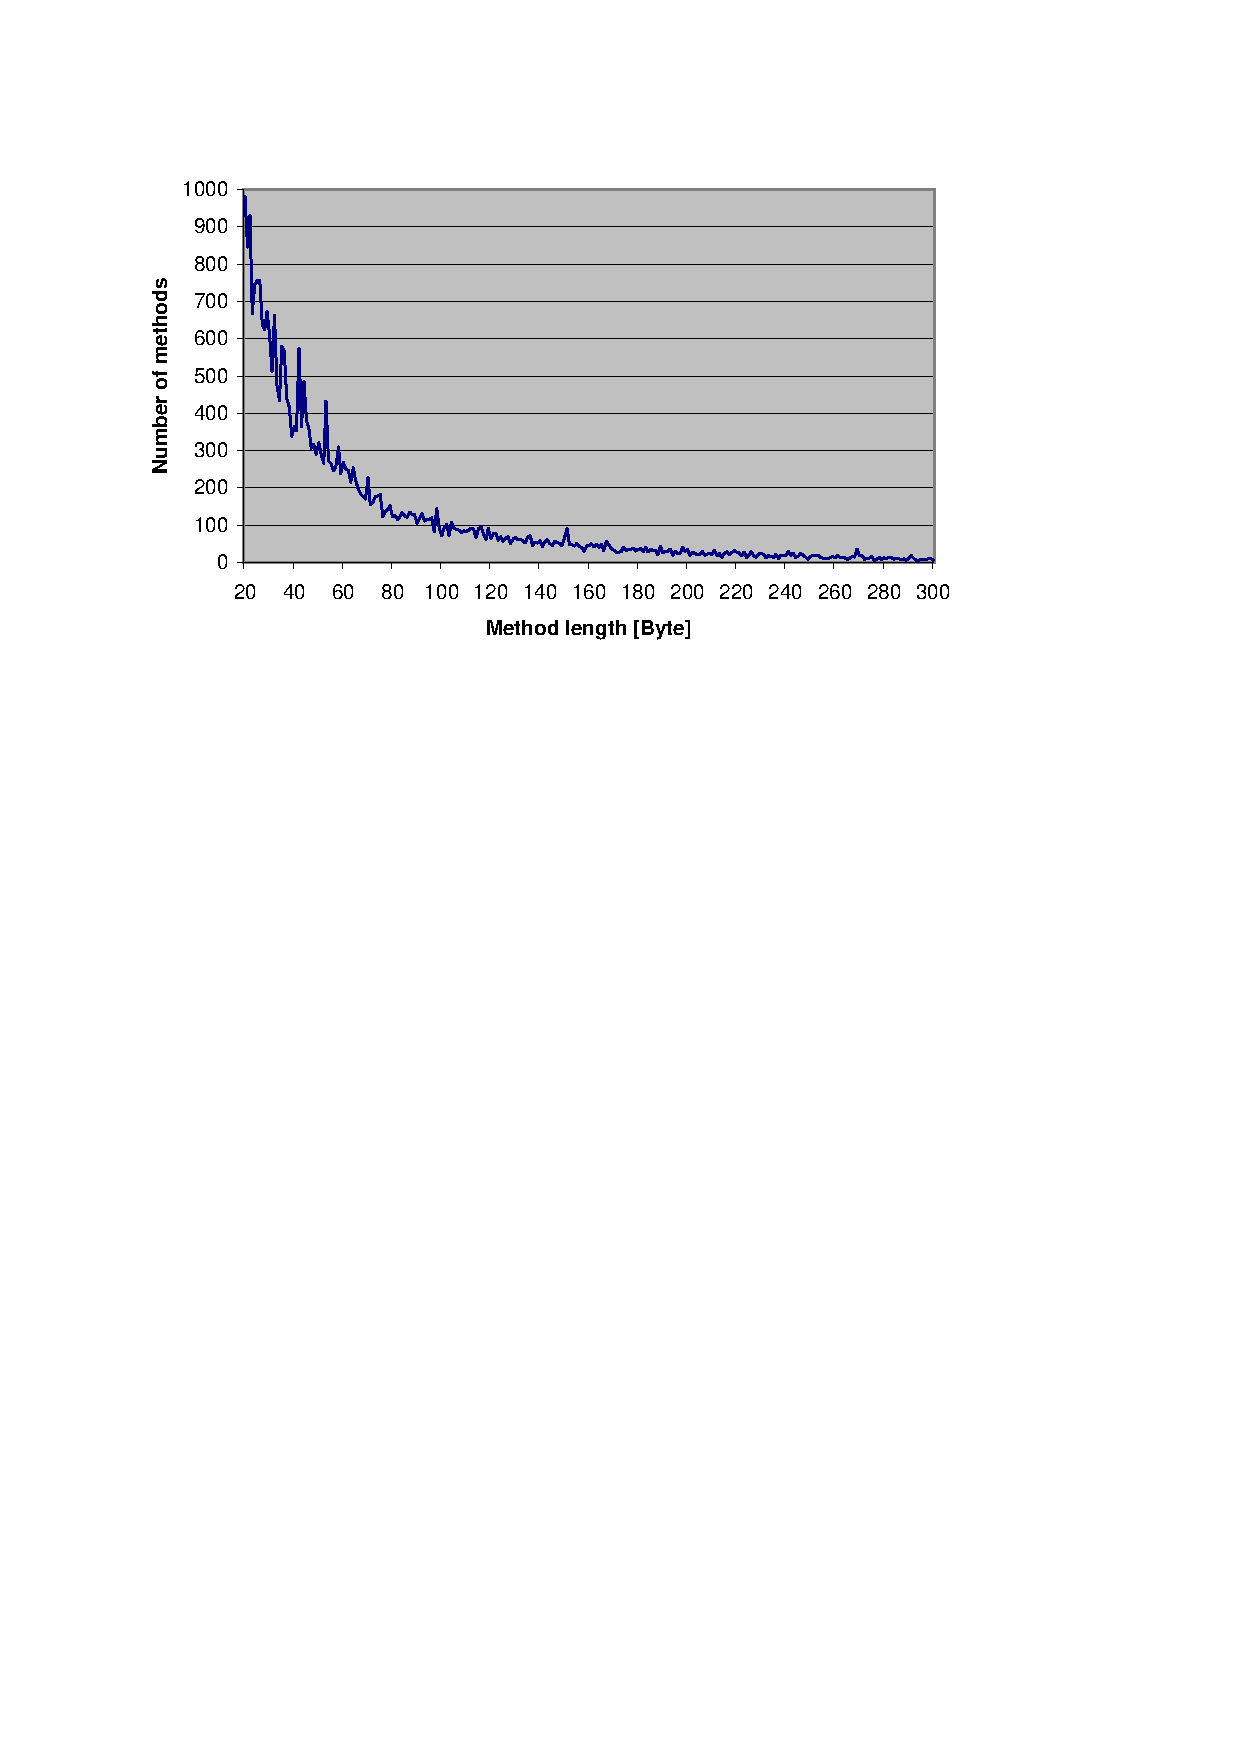
\includegraphics[width=\excelwidth]{arch/arch_meth300}
%    \caption[Static method count from the JDK 1.4 runtime library]
%    {Static method count from the JDK 1.4 runtime library.
%    The horizontal axis indicates the method size in bytes.}
%    \label{fig_java_meth300}
%\end{figure}
%
%In Figure~\ref{fig_java_meth32}, the distribution of small methods up
%to a size of 32 bytes is shown. \figurename~\ref{fig_java_meth300}
%shows the method count for methods up to 300 bytes. As expected, we
%see fewer methods as size increases. The method size of 5 bytes is
%very common. These methods are the typical setter and getter methods
%in object-oriented programming as shown in
%Listing~\ref{lst:arch:java:getval}. The method \code{getVal()}
%translates to three bytecodes of 1, 3 and 1 bytes in length
%respectively.
%
%
%\begin{lstlisting}[float, caption={Bytecodes for a getter method},label=lst:arch:java:getval]
%    private int val;
%
%    public int getVal() {
%        return val;
%    }
%
%    public int getVal();
%    Code:
%    0:   aload_0
%    1:   getfield        #2; //Field val:I
%    4:   ireturn
%\end{lstlisting}
%
%
%The static distribution of method sizes in an application (javac, the
%Java compiler) is quite similar to the distribution in the library.
%In the class file that contains the Java compiler, 98\% of the
%methods are smaller than 513 bytes, and the larger methods are class
%initializers.
%
%\subsection{Summary}
%
%In this section, we performed dynamic measurements on the JVM
%instruction set. We saw that more than 40\% of the executed
%instructions are local variables or constants loads onto the stack.
%This high frequency of stack access calls for an efficient
%implementation of the stack, as described in Section~\ref{sec:stack}.
%
%In addition, we have statically measured method sizes. Methods are
%typically very short. 30\% of the methods are shorter than 9 bytes
%and 99\% account for methods of up to 512 bytes. The maximum length
%is further limited by the definition of the class file. We will use
%this property in the proposed \emph{method cache} in
%Section~\ref{sec:cache}.
%
%Instruction-usage data is an important input for the design of a
%processor architecture, as seen in the following sections.
%
%
%%\subsection{Some more properties}
%%Number of local variables per method.
%
%
%%\subsubsection{Some Comments}
%%
%%* Clarification of the quick instructions
%
%%* A word about javac: absolute not optimized code generations.
%%Simplifies JIT, but not so good for Java processors or an
%%interpreting JVM
%
%%\dots CPI is not so easy to measure for the JVM. JVM = runtime
%%infrastructure (GC, new). What is measured with JIT?

\section{Summary}

Java is a unique combination of the language definition, a rich
class library and a runtime environment. A Java program is compiled
to bytecodes that are executed by a Java virtual machine. Strong
typing, runtime checks and avoidance of pointers make Java a
\emph{safe} language. The intermediate bytecode representation
simplifies porting of Java to different computer systems. An
interpreting JVM is easy to implement and needs few system
resources. However, the execution speed suffers from interpreting.
JVMs with a just-in-time compiler are state-of-the-art for desktop
and server systems. These compilers require large amounts of memory
and have to be ported for each processor architecture, which means
they are not the best choice for embedded systems. A Java processor
is the implementation of the JVM as a concrete machine. A Java
processor avoids the slow execution model of an interpreting JVM and
the memory requirements of a compiler, thus making it an interesting
execution system for Java in embedded systems.
